\section{Résultats}

\paragraph{Méthode statique}
Dans cette première partie, trois échantillons cylindriques ont été étudiés, un en laiton, un en acier et un dernier en magnésium. Les dimensions de ces échantillons ont été reportés dans le \autoref{tab:dimensions_echantillons_statique}. Les estimations pour les erreurs sont disponibles en \autoref{sec:erreurs}. Il est important de noter que le diamètre de l'échantillon de magnésium était deux fois plus grand que les deux autres échantillons. La mesure du diamètre a été réalisée à plusieurs niveaux sur la tige, puis la valeur moyenne a été retenue.

\begin{table}[h]
    \centering
    \begin{tabulary}{0.9\linewidth}{c C C}
        \toprule
        & $d$ [\si{\centi\meter}] & $D$ [\si{\centi\meter}] \\
        \midrule
        Laiton & $0.500 \pm 0.001$ & $9.951 \pm 0.005$ \\
        Acier & $0.506 \pm 0.001$ & $9.964 \pm 0.005$ \\
        Magnésium & $1.004 \pm 0.001$ & $9.940 \pm 0.005$ \\
        \bottomrule
    \end{tabulary}
    \caption{Dimensions des échantillons pour la méthode statique, où $d$ est le diamètre moyen de l'échantillon et $D$ le diamètre de la poulie}
    \label{tab:dimensions_echantillons_statique}
\end{table}

En faisant varier la masse suspendue à longueur d'échantillon constante $L=(25.0 \pm 0.1)$ \si{\centi\meter}, la \autoref{fig:statique_masse} a été obtenue. Une régression linéaire permet alors d'exprimer l'angle de déformation $\theta$ en fonction du poids $P=mg$. Les ordonnées à l'origine ont été négligées dans le calcul du module de cisaillement en raison de leur valeur négligeable devant la pente. Le procédé a été répété en faisant varier cette fois ci la longueur de l'échantillon à masse suspendu constante $m=(622 \pm 3)$ \si{\gram}. Les résulats sont reportés dans la \autoref{fig:statique_longueur}. La régression linéaire permet d'exprimer cette fois ci $\theta$ en fonction de $L$.

\begin{figure}[h]
    \centering
    \begin{subfigure}{0.45\linewidth}
        \centering
        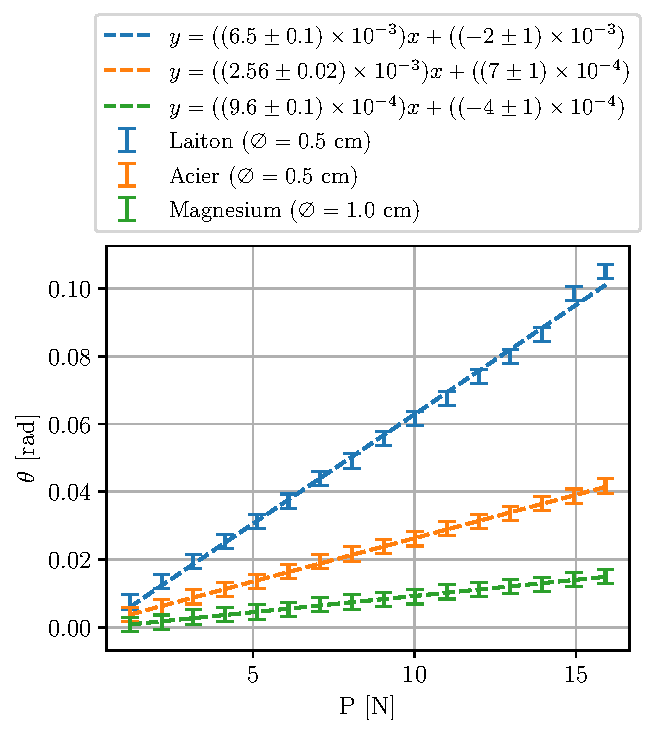
\includegraphics[width=\linewidth]{figures/methode_statique_masse.pdf}
        \caption{}
        \label{fig:statique_masse}
    \end{subfigure}
    \begin{subfigure}{0.45\linewidth}
        \centering
        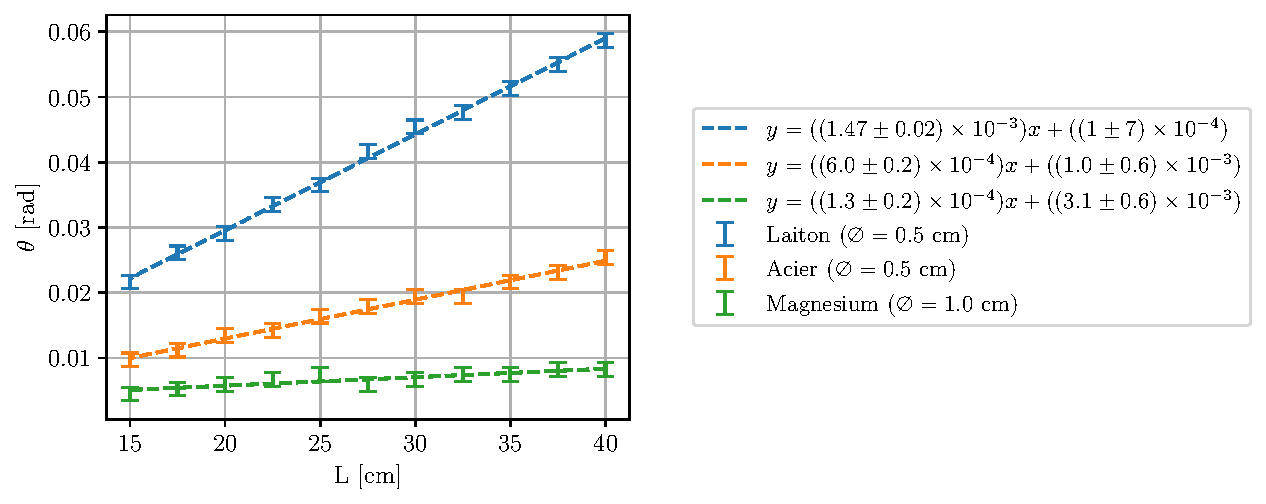
\includegraphics[width=\linewidth]{figures/methode_statique_longueur.pdf}
        \caption{}
        \label{fig:statique_longueur}
    \end{subfigure}
    \caption{Angle de déformation en fonction (a) du poids attaché et (b) de la longueur de l'échantillon pour la méthode statique}
\end{figure}

En utilisant l'\autoref{eq:module_cisaillement_statique}, le module de cisaillement $G$ pour chaque échantillon a été calculé et reporté dans le \autoref{tab:module_statique}. Les valeurs diffèrent légèrement aux valeurs de référence, mais restent cependant plutôt proches.

\begin{table}[h]
    \centering
    % \adjustbox{width=\linewidth}
    \begin{tabulary}{\linewidth}{c c c c c c}
        \toprule
        & $G_\textrm{ref}$ [\si{\giga\pascal}] & $G_P$ [\si{\giga\pascal}] & Écart relatif $G_P$ [\%] & $G_L$ [\si{\giga\pascal}] & Écart relatif $G_L$ [\%] \\
        \midrule
        Laiton & 37.3 & $31.1\pm0.7$ & $16.5 \pm 1.8$ & $33.4\pm0.7$ & $10.5 \pm 1.9$ \\
        Acier & 82.2 & $75\pm0.1$ & $8.0 \pm 1.3$ & $79\pm3$ & $3 \pm 3 $ \\
        Magnésium & 17.3 & $13.0\pm0.2$ & $25.0 \pm 1.1$ & $23\pm4$ & $35 \pm 22$ \\
        \bottomrule
    \end{tabulary}
    % \end{adjustbox}
    \caption{Modules de cisaillement obtenues pour chaque échantillon par la méthode statique en faisant varier le poids ($G_P$) et la longueur ($G_L$), comparé aux valeurs de référence}
    \label{tab:module_statique}
\end{table}

\paragraph{Méthode dynamique}
Ensuite, des échantillons de même composition mais de format differents ont été étudiés.les dimensions de ces échantillons en forme de fil ont été reportés dans le \autoref{tab:dimensions_echantillons_dynamique}. Encore une fois, l'échantillon de magnésium était plus épais que les deux autres échantillons. Le diamètre a été obtenu avec le même procédé que précedement.

\begin{table}[h]
    \centering
    \begin{tabulary}{0.9\linewidth}{c C C}
        \toprule
        & $d$ [\si{\milli\meter}] & $\ell$ [\si{\centi\meter}] \\
        \midrule
        Laiton & $1.127 \pm 0.008$ & $8.036 \pm 0.005$ \\
        Acier & $1.062 \pm 0.007$ & $7.996 \pm 0.005$ \\
        Magnésium & $2.035 \pm 0.007$ & $8.000 \pm 0.005$ \\
        \bottomrule
    \end{tabulary}
    \caption{Dimensions des échantillons pour la méthode dynamique, où $d$ est le diamètre moyen de l'échantillon et $\ell$ sa longueur}
    \label{tab:dimensions_echantillons_dynamique}
\end{table}

Le disque d'inertie avait pour masse $M=(2.991 \pm 0.1)$ \si{\kilo\gram} et rayon $R=(7.467 \pm 0.001)$ \si{\centi\meter}. Son moment d'inertie $I$ vaut alors $I=\int_V r^2 \dd V = \frac{MR^2}{2}$. Après la mise en mouvement du pendule de torsion, les oscillations ont été capturées pendant environ 60 \si{\second}. La \autoref{fig:dynamique} montre la décroissance de l'amplitude des oscillation pour chaque échantillon.

\begin{figure}[h]
    \centering
    \begin{subfigure}{0.45\linewidth}
        \centering
        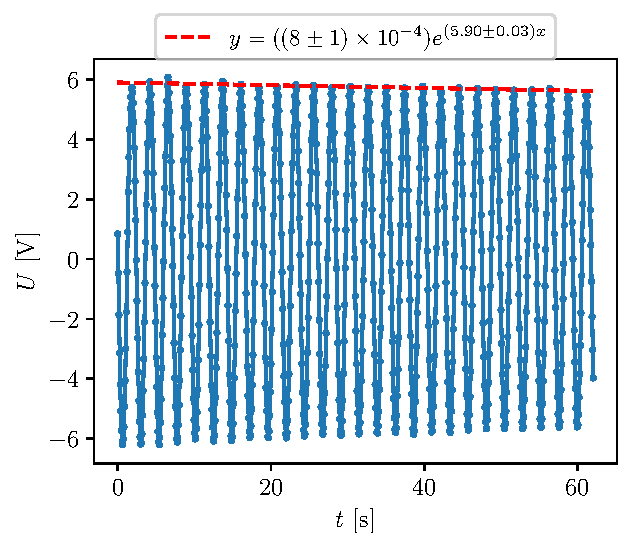
\includegraphics[width=\linewidth]{figures/laiton1.pdf}
        \caption{}
        \label{fig:dynamique_laiton}
    \end{subfigure}
    \begin{subfigure}{0.45\linewidth}
        \centering
        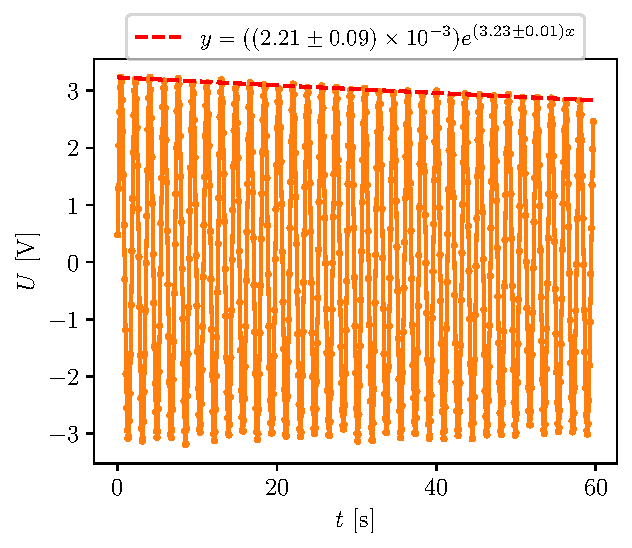
\includegraphics[width=\linewidth]{figures/acier1.pdf}
        \caption{}
        \label{fig:dynamique_acier}
    \end{subfigure}
    \begin{subfigure}{0.45\linewidth}
        \centering
        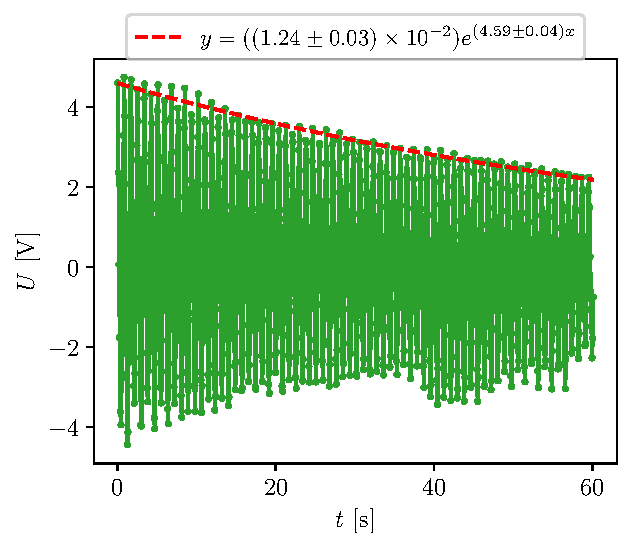
\includegraphics[width=\linewidth]{figures/magnesium3.pdf}
        \caption{}
        \label{fig:dynamique_magnesium}
    \end{subfigure}
    \caption{Décroissance de l'amplitude des oscillations des échantillons de (a) laiton, (b) acier et (c) magnésium}
    \label{fig:dynamique}
\end{figure}

Une régression avec une fonction de la forme $y = Ae^{-\lambda t}$ sur l'enveloppe des oscillations permet d'obtenir le coefficient d'amortissement $\lambda$ de l'échantillon. Afin d'ameillorer la précision, la moyenne de $\lambda$ sur 3 mesures a été prise. La periode $T$ des oscillations a été obtenue en considérant l'ensemble de la mesure, soit environ 30 periodes, permettant de trouver la periode avec une assez grande précision. L'\autoref{eq:module_cisaillement_dynamique} donne alors le module de cisaillement pour chaque échantillon. Les valeurs sont recensées dans le \autoref{tab:module_dynamique}.

\begin{table}[h]
    \centering
    \begin{tabulary}{0.9\linewidth}{c c c c c}
        \toprule
        & $T$ [\si{\second}] & $\lambda$ [\si{\per\second}] & $G_\textrm{dyn}$ [\si{\giga\pascal}] & Écart relatif $G_\textrm{dyn}$ [\%] \\
        \midrule
        Laiton & $3.5727 \pm 0.0005$ & $\left(9 \pm 2\right) \cdot 10^{-4}$ & $13.1 \pm 0.5$ & $65.0 \pm 1.3$ \\
        Acier & $2.7109 \pm 0.0004$  & $\left(2.51 \pm 0.04\right) \cdot 10^{-3}$ & $29 \pm 1$ & $65.0 \pm 1.3$ \\
        Magnésium & $1.2791 \pm 0.0002$ & $\left(1.31 \pm 0.03\right) \cdot 10^{-2}$ & $ 9.6 \pm 0.3$ & $44.7 \pm 1.9$ \\
        \bottomrule
    \end{tabulary}
    \caption{Periode d'oscillations, coefficient d'amortissement et modules de cisaillement $G_\textrm{dyn}$ obtenues pour chaque échantillon par la méthode dynamique, comparé aux valeurs de référence}
    \label{tab:module_dynamique}
\end{table}
